\documentclass[11pt]{report}

% Paquetes y configuraciones adicionales
\usepackage{graphicx}
\usepackage[export]{adjustbox}
\usepackage{caption}
\usepackage{float}
\usepackage{titlesec}
\usepackage{geometry}
\usepackage[hidelinks]{hyperref}
\usepackage{titling}
\usepackage{titlesec}
\usepackage{parskip}
\usepackage{wasysym}
\usepackage{tikzsymbols}
\usepackage{fancyvrb}
\usepackage{xurl}
\usepackage{hyperref}
\usepackage{subcaption}

\usepackage{listings}
\usepackage{xcolor}

\usepackage[spanish]{babel}

\newcommand{\subtitle}[1]{
  \posttitle{
    \par\end{center}
    \begin{center}\large#1\end{center}
    \vskip0.5em}
}

% Configura los márgenes
\geometry{
  left=2cm,   % Ajusta este valor al margen izquierdo deseado
  right=2cm,  % Ajusta este valor al margen derecho deseado
  top=3cm,
  bottom=3cm,
}

% Configuración de los títulos de las secciones
\titlespacing{\section}{0pt}{\parskip}{\parskip}
\titlespacing{\subsection}{0pt}{\parskip}{\parskip}
\titlespacing{\subsubsection}{0pt}{\parskip}{\parskip}

% Redefinir el formato de los capítulos y añadir un punto después del número
\makeatletter
\renewcommand{\@makechapterhead}[1]{%
  \vspace*{0\p@} % Ajusta este valor para el espaciado deseado antes del título del capítulo
  {\parindent \z@ \raggedright \normalfont
    \ifnum \c@secnumdepth >\m@ne
        \huge\bfseries \thechapter.\ % Añade un punto después del número
    \fi
    \interlinepenalty\@M
    #1\par\nobreak
    \vspace{10pt} % Ajusta este valor para el espacio deseado después del título del capítulo
  }}
\makeatother

% Configura para que cada \chapter no comience en una pagina nueva
\makeatletter
\renewcommand\chapter{\@startsection{chapter}{0}{\z@}%
    {-3.5ex \@plus -1ex \@minus -.2ex}%
    {2.3ex \@plus.2ex}%
    {\normalfont\Large\bfseries}}
\makeatother

% Configurar los colores para el código
\definecolor{codegreen}{rgb}{0,0.6,0}
\definecolor{codegray}{rgb}{0.5,0.5,0.5}
\definecolor{codepurple}{rgb}{0.58,0,0.82}
\definecolor{backcolour}{rgb}{0.95,0.95,0.92}

% Configurar el estilo para el código
\lstdefinestyle{mystyle}{
  backgroundcolor=\color{backcolour},   
  commentstyle=\color{codegreen},
  keywordstyle=\color{magenta},
  numberstyle=\tiny\color{codegray},
  stringstyle=\color{codepurple},
  basicstyle=\ttfamily\footnotesize,
  breakatwhitespace=false,         
  breaklines=true,                 
  captionpos=b,                    
  keepspaces=true,                 
  numbers=left,                    
  numbersep=5pt,                  
  showspaces=false,                
  showstringspaces=false,
  showtabs=false,                  
  tabsize=2
}

%==============================================================================
% Cosas para la documentación LateX
% % Sangría
% \setlength{\parindent}{1em}Texto

% % Quitar sangría
% \noindent

% % Punto
% \CIRCLE \ \ \textbf{Texto} \emph{algo}
% \begin{itemize}
%   \item \textbf{Negrita:} Texto
%   \item \textbf{Negrita:} Texto
% \end{itemize}

% % Introducir código
% \begin{center}
%   \begin{BVerbatim}
%     ... Código
%   \end{BVerbatim}
% \end{center}

% Poner una imagen
% \begin{figure}[H]
%   \centering
%   \includegraphics[scale=0.55]{img/}
%   \caption{Exportación de la base de datos en formato sql}
%   \label{fig:exportación de la base de datos en formato sql}
% \end{figure}

% Poner dos imágenes
% \begin{figure}[H]
%   \begin{subfigure}{0.5\textwidth}
%     \centering
%     \includegraphics[scale=0.45]{img/}
%     \caption{Texto imagen 1}
%   \end{subfigure}%
%   \begin{subfigure}{0.5\textwidth}
%     \centering
%     \includegraphics[scale=0.45]{img/}
%     \caption{Texto imagen 2}
%   \end{subfigure}
%   \caption{Texto general}
% \end{figure}

% % Poner una tabla
% \begin{table}[H]
%   \centering
%   \begin{tabular}{|c|c|c|c|}
%     \hline
%     \textbf{Campo 1} & \textbf{Campo 2} & \textbf{Campo 3} & \textbf{Campo 4} \\ \hline
%     Texto & Texto & Texto & Texto \\ \hline
%     Texto & Texto & Texto & Texto \\ \hline
%     Texto & Texto & Texto & Texto \\ \hline
%     Texto & Texto & Texto & Texto \\ \hline
%   \end{tabular}
%   \caption{Nombre de la tabla}
%   \label{tab:nombre de la tabla}
% \end{table}

% % Poner codigo de un lenguaje a partir de un archivo
% \lstset{style=mystyle}
% The next code will be directly imported from a file
% \lstinputlisting[language=Python]{code.py}

% “Texto entre comillas dobles”

%==============================================================================

\begin{document}

% Portada del informe
\title{Practica 12. Pentesting con Metasploit}
\subtitle{Seguridad de Sistemas Informáticos}
\author{Carlos Pérez Fino \texttt{alu0101340333@ull.edu.es} \and Cheuk Kelly Ng Pante \texttt{alu0101364544@ull.edu.es}}
\date{\today}

\maketitle

\pagestyle{empty} % Desactiva la numeración de página para el índice

% Índice
\tableofcontents

% Nueva página
\cleardoublepage

\pagestyle{plain} % Vuelve a activar la numeración de página
\setcounter{page}{1} % Reinicia el contador de página a 1

% Secciones del informe
% Capitulo 1
\chapter{Instalación de paquetes de Kali Linux en una máquina Debian}
Para instalar los paquetes básicos de Kali Linux en una máquina \emph{Debian} hemos usado un script creado por un usuario en GitHub llamado \emph{Katoolin3} \cite{0}. 
Este script nos permite instalar los paquetes básicos de Kali Linux en una máquina Debian o Ubuntu. Para instalarlo, debemos tener instalado los siguientes requisitos:
\begin{itemize}
  \item \textbf{apt como gestor de paquetes}
  \item \textbf{Privilegios de superusuario}
  \item \textbf{sh y bash}
  \item \textbf{Python \texttt{>=} 3.5:} \texttt{sudo apt install python3}
  \item \textbf{Git:} \texttt{sudo apt install git}
  \item \textbf{Python3-apt:} \texttt{sudo apt install python3-apt}
\end{itemize}

Una vez instalados los requisitos, procedemos a la instalación de \emph{Katoolin3}:
\begin{verbatim}
git clone https://github.com/s-h-3-l-l/katoolin3;
cd katoolin3;
sudo chmod +x install.sh;
\end{verbatim}

Ya instalado, entramos como root con \emph{sudo su} y ejecutamos lo siguiente para poder descargar la clave pública desde la URL proporcionada y luego agregarla 
al sistema como una clave GPG válida y así poder descargar los paquetes de Kali Linux y verificar la autenticidad de los paquetes durante las operaciones de instalación:
\begin{verbatim}
wget -q -O - https://archive.kali.org/archive-key.asc | apt-key add;
\end{verbatim}

Antes que nada, comprobamos con el comando \texttt{sudo apt-key list} que se ha añadido la clave de Kali Linux:
\begin{figure}[H]
  \centering
  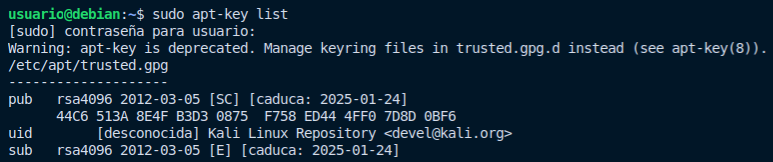
\includegraphics[scale=0.5]{img/apt-key_list.png}
  \caption{Imagen del comando \texttt{sudo apt-key list}}
\end{figure}

ya comprobada la clave, procedemos a comentar la línea 22 del script \emph{install.sh} para que no de error como se muestra en la figura \ref{fig:script}
\begin{figure}[H]
  \centering
  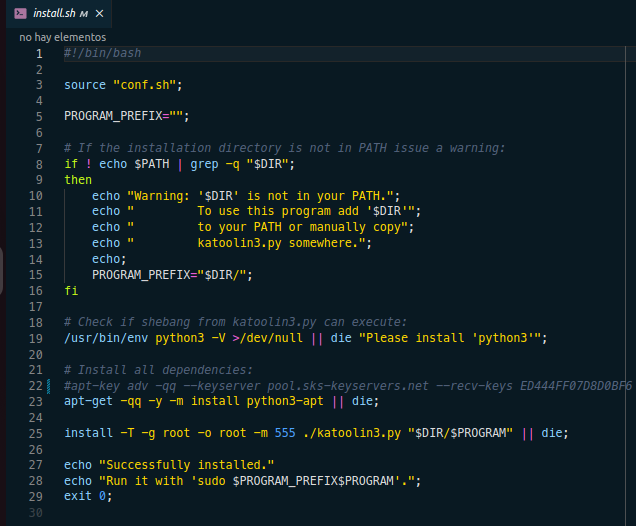
\includegraphics[scale=0.5]{img/comment_script.png}
  \caption{Imagen del script \emph{install.sh}}
  \label{fig:script}
\end{figure}

Una vez comentada la línea, ejecutamos el script de instalación:
\begin{verbatim}
sudo ./install.sh
\end{verbatim}

Una vez hecha la instalación procedemos a ejecutar el script \emph{katoolin3.py} para poder instalar los paquetes de Kali Linux:
\begin{verbatim}
sudo python3 katoolin3.py
\end{verbatim}

Cuando ejecutemos el script nos aparecerá un menú como el de la figura \ref{fig:menu}:
% \begin{figure}[H]
%   \centering
%   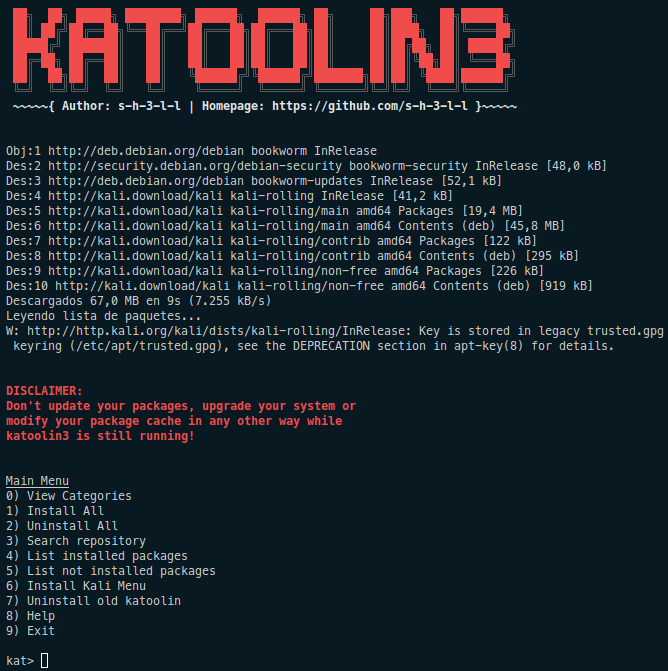
\includegraphics[scale=0.5]{img/menu.png}
%   \caption{Imagen del menú de \emph{katoolin3.py}}
%   \label{fig:menu}
% \end{figure}

Para instalar los paquetes básicos de Kali Linux, seleccionamos la opción 0 y nos aparecerá un menú como el de la figura \ref{fig:menu2} y en el nuevo
menú seleccionamos la opción 0 para instalar las herramientas de explotación y nos saldrá otro menú y seleccionamos la opción 20 para instalar todas las herramientas:
\begin{figure}[H]
  \centering
  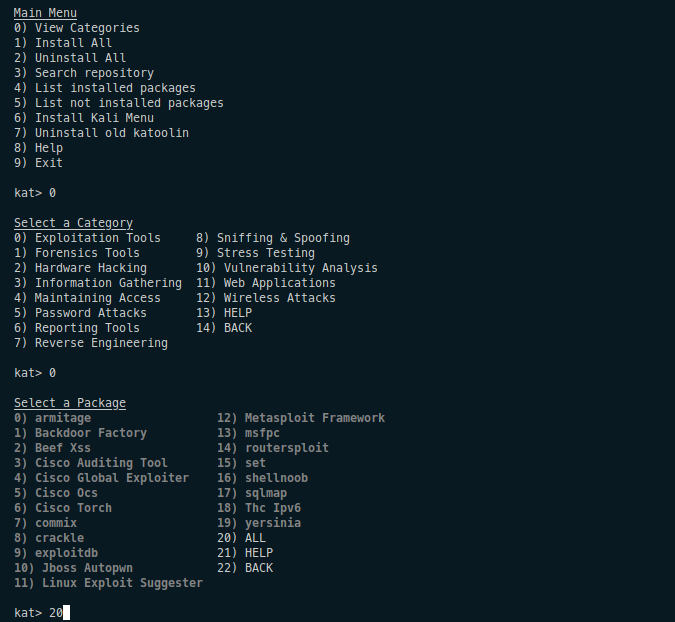
\includegraphics[scale=0.4]{img/menu2.png}
  \caption{Imagen del menú de \emph{katoolin3.py}}
  \label{fig:menu2}
\end{figure}


% Capitulo 2
\chapter{Capitulo 2}
% 2.1
\section{Seccion 2.1}

\chapter{Bibliografía} % En formato APA
\begin{thebibliography}{99}
  \bibitem{0} s-h-3-l-l. (2019). Katoolin3. Github. Recuperado de \url{https://github.com/s-h-3-l-l/katoolin3}
\end{thebibliography}

\end{document}
